\documentclass[undgrad,numbers]{Controle/DES}
\usepackage[utf8]{inputenc}
\usepackage{amsmath,amssymb}
\usepackage{epigraph}
\usepackage{hyperref}
\usepackage{indentfirst}
%\usepackage{csquotes}
\usepackage{tikz}
\usepackage{longtable}
\usepackage[refpage]{nomencl}
\usepackage{lettrine}
\usepackage{multirow}
\usepackage{array}
\usepackage{tikz}
\usepackage[RPvoltages, american, cuteinductors,smartlabels]{circuitikz}
%\usepackage[]{circuitikz}
\usepackage{color, colortbl}
\usepackage{ctable}
%\setlength{\arrayrulewidth}{0.5mm}
\usepackage[document]{ragged2e}
\usepackage{lmodern}
\usepackage{pdfpages}
\usepackage[font=footnotesize,labelfont=bf]{caption}
\usepackage{fancyhdr}
\usepackage{ifthen}
\usepackage[alf]{abntex2cite}

\pagestyle{fancyplain}
\fancyhf{}
\fancyhead[R]{\thepage}
\renewcommand{\headrulewidth}{0pt}

\makelosymbols
\makeloabbreviations
\justifying

\begin{document}
  \title{Projeto Pedagógico do Curso de Engenharia Eletrônica} %Máximo de 4 linhas
  \foreigntitle{My great title in english here}
  \author{Primeiro nome}{Sobrenome1 Sobrenome2} %Nome do(a) autor(a)

  \advisor{Prof.}{Nome do(a) Orientador(a)}{D.Sc.} %Nome do(a) orientador(a)
  \newcommand{\exinsto}{Universidade Federal de Pernambuco} %IES do Orientador

  \examiner{Prof.}{Nome do(a) primeiro(a) examinador(a)}{D.Sc.}
  \newcommand{\exinstum}{Universidade Federal de Pernambuco} %IES do primeiro examinador

  \examiner{Prof.}{Nome do(a) segundo(a) examinador(a)}{Ph.D.}
  \newcommand{\exinstdois}{Universidade Federal de Pernambuco} %IES do segundo examinador

  \coadvisor{Prof.}{Nome do(a) Coorientador(a)}{D.Sc.}
  % Coloque % no segundo examinador, caso não tenha.
  % Coloque % no Coorientador, caso não tenha.

  \department{DES-ELE} % DES-TEL para Telecomunicações
  \date{\the\month}{\the\year}

  \newcommand{\Datadadefesa}{xx/xx/20xx}%Coloque a data da defesa dd/mm/aaaa

  \mainmatter
  %\thispagestyle{empty}
\dedication{A alguém muito importante}

\textcolor{red}{[Dedicatória é um elemento opcional]}
 %Dedicatória
  %\thispagestyle{empty}
\Huge
\textbf{Agradecimentos}
\normalsize
\vspace{1cm}

%Início dos agradecimentos
Muitos agradecimentos a várias pessoas aqui.

\textcolor{red}{[Agradecimentos é um elemento opcional]} %Agradecimentos
  %\thispagestyle{empty}
\mbox{}\vfill
\epigraph{Uma frase de efeito aqui dita por outra pessoa}{O autor da epígrafe}
\textcolor{red}{[Epígrafe é um elemento opcional]}
 %Epígrafe
  %\begin{abstract}

O resumo do trabalho tem a finalidade de dar uma visão rápida ao leitor, para que ele possa decidir sobre a conveniência da leitura do texto inteiro. Ele tem que ser totalmente fiel ao trabalho e não pode conter nenhuma informação que não conste do texto integral. A primeira frase do resumo deve ser significativa, explicando o tema principal do documento. Não devem constar do resumo citação de autores, tabelas e figuras. O resumo precisa estar contido em um único parágrafo e em uma única página. De acordo com a norma da ABNT NBR 6028, o resumo deve conter até 500 palavras. Ao final, devem ser incluídas, por recomendação, entre três e cinco palavras-chave.

\palavraschave{Suspendisse; orci; iaculis; dignissim.}\\
\textcolor{red}{Obs: Palavras-chave separadas por ponto e vírgula, ponto no final e em minúsculas (com exceção dos substantivos próprios e nomes científicos).}

\end{abstract}
 %Resumo em português
  %\begin{foreignabstract}

Class aptent taciti sociosqu ad litora torquent per conubia nostra, per inceptos himenaeos. Nullam tempus interdum arcu, sed ullamcorper ipsum tempor et. Integer fermentum aliquam arcu, vel condimentum purus tincidunt id. Ut purus est, lobortis eu nisi sed, efficitur aliquam neque. Vestibulum vestibulum malesuada ante, vitae molestie erat ullamcorper vel. Mauris semper vestibulum est id bibendum. Quisque vehicula at purus id dapibus. Sed ornare, est ut luctus ultricies, odio justo pretium ipsum, et maximus lectus orci in libero. Sed sit amet lacus at odio ullamcorper convallis sit amet sed lacus.

\keywords{Digital Communications; Acoustic Communications; FPGA; Hardware Coprocessor.}\\
\textcolor{red}{Obs: Palavras-chave em inglês separadas por ponto e vírgula, ponto no final e em minúsculas (com exceção dos substantivos próprios e nomes científicos).}

\end{foreignabstract}
 %Resumo em inglês 

  %\addtocontents{toc}{\protect\thispagestyle{empty}}

\cleardoublepage
\begingroup
  \makeatletter
  \let\ps@plain\ps@empty
  \makeatother

  \pagestyle{empty}
  \tableofcontents
  \listoffigures %Gerar a lista de Ilustrações
  \listoftables %Gerar a lista de Tabelas
  \cleardoublepage

  %\thispagestyle{empty}
\Huge
\textbf{Lista de Símbolos}
\normalsize
\vspace{1cm}

\begin{longtable}{lr}
A&\dotfill     Ampère\\
e&\dotfill      Constante de Euler ou Constante de Napier\\
E&\dotfill      Energia
\end{longtable}
  %Gerar a lista de Símbolos
  %\thispagestyle{empty}
\Huge
\textbf{{Lista de Abreviações}}
\normalsize
\vspace{1cm}

\begin{longtable}{lr}
    AD&\dotfill Analógico-para-Digital\\
    bps	&\dotfill bits por segundo  \\
    CI	&\dotfill Circuito Integrado  \\
    DA	&\dotfill Digital-para-Analógico
\end{longtable}
  %Gerar a lista de Abreviaturas
\endgroup

  \pagestyle{plain}
  \chapter{Histórico da UFPE e do Curso de Engenharia Eletrônica}
\label{cap:um}

A fundação da Universidade do Recife (UR), em 11 de agosto de 1946, dá início à história da Universidade Federal de Pernambuco. A UR foi criada por meio do Decreto-Lei da Presidência da República nº 9.388, de 20 de junho de 1946, e reunia a Faculdade de Direito do Recife, fundada em 1827, a Escola de Engenharia de Pernambuco (1895), a Faculdade de Medicina do Recife (1927), com as escolas anexas de Odontologia (1913) e Farmácia (1903), a Escola de Belas Artes de Pernambuco (1932) e a Faculdade de Filosofia do Recife (1941). Os Institutos de Geociências, Física, e Ciências do Homem, entre outros, foram criados na década de 60.

A Universidade do Recife foi federalizada pela Lei nº 4.759, de 20 de agosto de 1965. Então, a UR passou a integrar o grupo de instituições federais do novo sistema de educação do país, e recebeu a denominação de Universidade Federal de Pernambuco (UFPE), autarquia vinculada ao Ministério da Educação.

Estabelecida em 1975, a atual estrutura de centros e departamentos da UFPE compreende 13 centros acadêmicos, sendo 11 no Recife, um em Caruaru (campus do Agreste, a 140 km do Recife) e outro em Vitória de Santo Antão (a 55 km do Recife). São ofertados atualmente 104 cursos de graduação presenciais, sendo 86 cursos no campus Recife, 12 no campus do Agreste, e 6 no campus de Vitória de Santo Antão, com um total de 28.989 alunos matriculados (dados do semestre 2020.1). Além dos cursos presenciais, a UFPE oferece 5 cursos de graduação a distância, com 449 alunos matriculados. A UFPE oferece ainda 152 cursos de pós-graduação stricto sensu, sendo 74 Mestrados Acadêmicos, 18 Mestrados Profissionais e 54 Doutorados, assim como 22 cursos de pós-graduação lato sensu presenciais (especializações). Há também 362 projetos de extensão voltados para a comunidade.

A estrutura física da UFPE é complementada, no campus Recife, por uma Biblioteca Central, 10 bibliotecas setoriais, o Núcleo de Tecnologia da Informação, a Editora UFPE, o Núcleo de Educação Física e Desportos, o Laboratório de Imunopatologia Keiso-Asami, o Núcleo de Saúde Pública e o Hospital das Clínicas. Na cidade do Recife, encontra-se o Núcleo de Educação Continuada, o Departamento de Extensão Cultural, o Memorial da Universidade de Medicina, o Teatro Joaquim Cardozo e o Núcleo de Rádio e Televisão. Em cidades vizinhas a Recife, duas unidades avançadas de pesquisa completam a estrutura da UFPE: Estação Ecológica Serra dos Cavalos (em Caruaru), e Estação de Itamaracá.

A unidade responsável pela manutenção do Curso de Engenharia Eletrônica na UFPE será o Departamento de Eletrônica e Sistemas — DES. O DES teve origem no antigo Departamento de Engenharia Elétrica (DEE) da UFPE. Em 1950 foi graduada a primeira turma de engenheiros eletricistas formados no DEE da UFPE.

Um programa conjunto com o Departamento de Física nessa época, com o apoio inicial do BNDE/TELEBRÁS e posteriormente da FINEP, fortaleceu o grupo de Eletrônica. Em 1977 foi implementado no DEE o programa de Pós-Graduação com a criação do Mestrado. Foram iniciadas atividades de pesquisa e criadas novas disciplinas nos cursos de graduação e pós-graduação em Arquitetura e Organização de Computadores, Bioeletrônica, Processamento de Sinais de Vídeo, Sistemas de Comunicações, Sistemas de Controle, Reconhecimento de Padrões, Teoria da Informação, Decisão e Planejamento, Fontes não Convencionais de Energia e Dispositivos de Microondas.  Como consequência, a área de Eletrônica e Sistemas, que inicialmente representava uma pequena fração das atividades do DEE, passou a constituir uma parte substancial das atribuições deste Departamento. Isso exigiu das referidas áreas uma maior representatividade, resultando, então, na criação do Departamento de Eletrônica e Sistemas (DES) em outubro de 1979.

Atualmente o DES conta com vinte e nove professores, todos doutores e em regime de Dedicação Exclusiva. Sete professores do DES são bolsistas de produtividade em pesquisa do CNPq. A maioria dos professores participa dos quatro principais grupos de pesquisa do DES credenciados pela UFPE e CNPq: Eletrônica, Engenharia da Informação, Fotônica e Comunicações. Estes grupos mantêm laboratórios e atuam em ensino, pesquisa e extensão nas áreas de controle, processamento de sinais, eletrônica analógica e digital, comunicações móveis, comunicações ópticas, códigos corretores de erros, criptografia, teoria da informação, propagação de ondas eletromagnéticas, antenas, dispositivos de micro-ondas, inteligência artificial, sistemas embarcados e outras. Portanto, a Engenharia Eletrônica constitui-se em uma vocação natural do DES.

Atualmente o DES responde pelos Cursos de Graduação em Engenharia Elétrica/Eletrônica\footnote{A partir de 2010, o curso Engenharia Elétrica/Eletrônica passou a se chamar Engenharia Eletrônica com a criação do perfil 4506 (cópia exata do perfil 4505).
} (conhecido como Engenharia Eletrônica) e Engenharia de Telecomunicações, e contribui fortemente com os Cursos de Graduação em Engenharia Elétrica, Engenharia de Controle e Automação, Engenharia Biomédica e Engenharia da Computação da UFPE.
 %Gerar o Capítulo 1
  \chapter{Justificativa}
\label{cap:dois}

A presença da tecnologia na sociedade humana em todo o mundo vem aumentando ano a ano, expandindo a setores antes alheios a ela. Seja para tornar sistemas e processos mais eficientes, seja para proporcionar distração a indivíduos, a sua influência é sentida cada vez mais profundamente. Na automação de sistemas, na comunicação de informações e no desenvolvimento de novos equipamentos, o impacto do uso da tecnologia vem sendo impressionante.

Às áreas tradicionais de eletrônica e telecomunicações, novos campos de atuação vêm se somando a cada ano. Desenvolvimento de instrumentos biomédicos, implementação de redes de sensores e aplicações em fontes alternativas de energia são fortes exemplos deste fenômeno.

Por outro lado, o estado de Pernambuco vem recebendo investimentos vultosos para o desenvolvimento do seu parque tecnológico, e várias indústrias dos mais diversos setores têm se instalado na região, em particular em SUAPE. Como toda indústria moderna, independente do setor, utiliza maquinaria automatizada, esta expansão do parque industrial vem aumentando a demanda por serviços técnicos especializados na área de eletrônica. Além disso, no estado também existem diversas empresas de desenvolvimento de equipamentos eletrônicos, empresas de desenvolvimento de softwares e empresas de prestação de serviços que necessitam de engenheiros eletrônicos capacitados para realizar os seus serviços de forma eficiente, competente e segura.

O engenheiro eletrônico deverá então ser capaz de estar envolvido neste processo através do projeto, desenvolvimento, testes e implantação de dispositivos, sensores e sistemas eletrônicos, assim como da prestação de serviços especializados e da manutenção e operação de sistemas. Além disso, o engenheiro hoje em dia é solicitado a considerar questões sociais e ambientais, valorizando assim o ser humano e o meio ambiente. Ele deve entender a complexidade dos problemas ambientais e, em consequência, a necessidade de se desenvolver o senso crítico e as habilidades necessárias para resolver estes problemas e construir sociedades socialmente justas, sustentáveis e ecologicamente equilibradas.

A sua formação, portanto, é de extrema importância para o desenvolvimento da região. Nesse contexto, o curso de Engenharia Eletrônica da Universidade Federal de Pernambuco, além de propiciar esta formação, busca desenvolver o trabalho de pesquisa e investigação científica, integrar os conhecimentos profissionais com a estrutura intelectual de cada geração, estimular o conhecimento dos problemas atuais mundiais, nacionais e regionais, ensinar uma capacidade de decisão crítica para destacar os valores éticos e a responsabilidade social, fomentar e inserir o futuro profissional na sociedade em que vive, apresentando-lhes os desafios a serem enfrentados e as suas responsabilidades com o desenvolvimento social, condição necessária para a formação de um profissional ético e um cidadão integral.

A elaboração do presente documento se justifica, também, pela necessidade de resposta a uma demanda natural de áreas como a Engenharia: a constante atualização dos instrumentos relacionados às práticas educacionais nesse contexto, em função de sua rápida e dinâmica evolução sob diversos aspectos. A proposição de um novo projeto pedagógico, associado a um perfil curricular moderno e sincronizado principalmente com o mercado, vem preencher diversas lacunas surgidas ao longo dos últimos anos, conforme delineado nas seções que se seguem.

Por último, este PPC visa adequar o Curso de Engenharia Eletrônica a duas novas resoluções para o ensino superior. A primeira é a Resolução n° 02, de 24 de abril de 2019, do Conselho Nacional de Educação/Câmara de Educação Superior (CNE/CES), que estabelece as novas Diretrizes Curriculares Nacionais do Curso de Graduação em Engenharia. A segunda é a Resolução nº 7, de 18 de dezembro de 2018, do Conselho Nacional de Educação /Câmara de Educação Superior (CNE/CES), que estabelece as diretrizes para a extensão na Educação Superior brasileira e regulamenta a reserva mínima de dez por cento do total de créditos exigidos para a graduação em programas e projetos de extensão universitária, a chamada curricularização da extensão.
 %Gerar o Capítulo 2
  \chapter{Marco Teórico}
\label{cap:tres}

O presente projeto pedagógico fundamenta-se na concepção epistemológica de que o “Engenheiro”, sendo criador e aplicador das mais diferentes tecnologias para o benefício da sociedade, é o elemento principal que poderá contribuir como profissional e cidadão para a solução de problemas relacionados à Elétrica / Eletrônica que afligem a coletividade. É um pressuposto que este profissional tenha a capacidade de assimilar outros conhecimentos que o tornem capaz de considerar o ser humano como elemento central de todas as suas atenções, modificando aqueles costumes e culturas que contrariem a necessidade de preservação, comunicação e bem estar de seus semelhantes.

A concepção do currículo do curso de Engenharia Eletrônica e as diretrizes do seu processo adaptativo/evolutivo têm como pilar fundamental a aplicação metodologias de ensino/aprendizagem que promovam a construção do saber crítico e reflexivo. Os componentes curriculares devem proporcionar meios para construção de um novo conceito ou consolidação de um conceito objeto do estudo, com espaço para construção coletiva e participativa.  A metodologia de aprendizagem também deve ser aprimorada a partir da autoavaliação contínua do curso.

Em adição a preocupação de desenvolvimento de uma base sólida do estudante, o curso não descuida dos aspectos relativos aos valores éticos e morais, prevendo dentro o componente curricular obrigatório “sociologia e meio ambiente” a discussão de temáticas importantes para formação do cidadão em suas dimensões mais amplas, como fatores culturais sociais, cultura, interação social, grupos sociais,  normas sociais e Relações Étnico raciais os quais são essenciais para a formação do cidadão consciente de seu papel na sociedade, bem como para a construção de consciência livre de preconceito e com entendimento das particularidades culturais, devido ao conhecimento da história dos diferentes grupos culturais, incluindo a história da cultura Afro-brasileira.

O curso favorece ao desenvolvimento do espírito empreendedor presente em cada aluno, bem como permite a conscientização para o uso equilibrado dos elementos presentes nos sistemas produtivos, em favor do meio ambiente e de uma cultura que promova a sustentabilidade com os olhos voltados para as especificidades regionais.

Oportunidades de aprimoramento da formação acadêmica são proporcionadas durante todo o trajeto dos estudantes no curso, os quais podem participar de iniciação científicas, de projetos de pesquisas, de monitorias, bem como de programas de intercâmbio. Tais ações são incentivadas, bem como instruídas pela coordenação do curso.

Além do ensino e da pesquisa, os alunos do curso têm participação em atividades de extensão, as quais são oferecidas por órgão específico dentro da universidade. É importante destacar que as atividades de extensão se constituem num importante e eficaz instrumento institucional que promove a troca de saberes e a integração com a sociedade. Além disso, ao mesmo tempo em que beneficia a população, contribuindo para a melhoria da qualidade de vida, inclusão sócio-produtiva e defesa do meio ambiente, as ações extensionistas – que incluem atividades técnicas, científicas, culturais e artísticas – propiciam ao estudante a oportunidade para um aprendizado teórico-prático contextualizado, desenvolvimento cultural, responsabilidade social e formação da cidadania.

Por tudo que foi colocado, o currículo ora proposto pelo curso estabelece a integração entre ensino, pesquisa e extensão universitária como metas constantes e integradas. 
 %Gerar o Capítulo 3
  \chapter{Objetivos}
\label{cap4}

O objetivo do curso de Engenharia Eletrônica é formar profissionais com uma sólida capacidade técnica aliada a uma visão ética, ambientalista e humanista para atender à demanda tecnológica e científica do mercado local e global, incluindo a carreira acadêmica. 

Os objetivos específicos que se pretende alcançar, em consonância com as diretrizes curriculares (Anexo 1), são:
\begin{enumerate}
	\item[$\bullet$]capacitar o discente a:
\begin{itemize}
	\item[-] elaborar, executar e analisar projetos técnicos e científicos;
	\item[-]acompanhar as evoluções tecnológicas da Engenharia Eletrônica;
	\item[-]desenvolver pesquisas em eletrônica;
	\item[-]atuar administrativamente no desempenho de funções relacionadas à Engenharia Eletrônica.
\end{itemize}
	\item[$\bullet$]oferecer um ensino centrado no discente e voltado para os resultados do aprendizado;
	\item[$\bullet$]enfatizar a solução de problemas de engenharia;
	\item[$\bullet$]formar profissionais adaptáveis às rápidas evoluções tecnológicas;
	\item[$\bullet$]oportunizar uma sólida formação geral;
	\item[$\bullet$]proporcionar uma articulação com a pós-graduação com ênfase na inovação;
	\item[$\bullet$]incentivar a interdisciplinaridade.
\end{enumerate}
 %Gerar o Capítulo 4
  \chapter{Perfil Profissional do Egresso}
\label{cap5}

O perfil dos egressos do curso de Engenharia Eletrônica da UFPE compreenderá uma sólida formação técnica-científica e profissional geral que capacite-o a absorver e desenvolver novas tecnologias, estimulando a sua atuação crítica e criativa na identificação e resolução de problemas, considerando seus aspectos políticos, econômicos, sociais, ambientais e culturais, com visão ética, humanística e cidadã, em atendimento às demandas da região e da sociedade como um todo. O profissional a ser formado na UFPE em Engenharia Eletrônica terá as seguintes atuações, de acordo com o CONFEA em sua Resolução n.º 218, Art. 9º: “o desempenho das atividades [...] referentes a materiais elétricos e eletrônicos; equipamentos eletrônicos em geral; sistemas de comunicação e telecomunicações; sistemas de medição e controle elétrico e eletrônico; seus serviços afins e correlatos” (Anexo 1).
 %Gerar o Capítulo 5
  \chapter{Campo de atuação do profissional}
\label{cap6}

O Engenheiro Eletrônico da UFPE será um profissional de formação generalista, que atua na área de materiais eletro-eletrônicos; sistemas de medição e de controle eletro-eletrônico; desenvolvimento de sistemas, produtos e equipamentos eletrônicos, sistemas embarcados, conversores, equipamentos biomédicos e informática médica. Estuda, projeta e especifica materiais, componentes, dispositivos e equipamentos eletro-eletrônicos, eletromecânicos, magnéticos, ópticos, de instrumentação, sensores e atuadores de transmissão e recepção de dados, de áudio/vídeo, de segurança patrimonial e de eletrônica embarcada. Planeja, projeta, instala, opera e mantém sistemas e instalações eletrônicas, equipamentos, dispositivos e componentes odonto-médico-hospitalares e de instrumentação biomédica, sistemas de medição e instrumentação eletro-eletrônica, de acionamentos de máquinas, de controle eletrônico e de automação, e de sistemas eletrônicos embarcados. Coordena e supervisiona equipes de trabalho, realiza estudos de viabilidade técnico-econômica, executa e fiscaliza obras e serviços técnicos; e efetua vistorias, perícias e avaliações, emitindo laudos e pareceres. Em suas atividades, considera a ética, a segurança, a legislação e os impactos ambientais.
 %Gerar o Capítulo 6
  \chapter{Competências, atitudes e habilidades}
\label{cap7}

Com a sempre presente tendência da tecnologia de ser cada vez mais aplicada aos mais diversos produtos e sistemas, o Engenheiro Eletrônico se encontra no centro de uma grande revolução tecnológica com o potencial para prover profundos benefícios para a sociedade. Criação de sistemas de controle eletrônico, instrumentos de telemetria, processamento digital e analógico, desenvolvimento de computadores, robótica e soluções eletrônicas para a indústria são algumas das áreas com grandes expectativas para o futuro. Assim, para ser capaz de trabalhar com sucesso neste ambiente, não basta para o Engenheiro Eletrônico dominar apenas o conhecimento técnico, é preciso também que ele domine várias habilidades gerais. A formação do Engenheiro Eletrônico terá por objetivo dotar o profissional dos conhecimentos requeridos para o exercício das seguintes competências e habilidades gerais:
\begin{enumerate}
\item[$\bullet$] aplicar conhecimentos matemáticos, científicos, tecnológicos e instrumentais à engenharia elétrica / eletrônica;
\item[$\bullet$] projetar e conduzir experimentos e interpretar resultados;
\item[$\bullet$] conceber, projetar e analisar sistemas, produtos e processos;
\item[$\bullet$] planejar, supervisionar, elaborar e coordenar projetos e serviços de engenharia elétrica/eletrônica;
\item[$\bullet$] identificar, formular e resolver problemas de engenharia elétrica/eletrônica;
\item[$\bullet$] desenvolver e/ou utilizar novas ferramentas e técnicas;
\item[$\bullet$] supervisionar a operação e a manutenção de sistemas elétricos/eletrônicos;
\item[$\bullet$] avaliar criticamente a operação e a manutenção de sistemas elétricos/eletrônicos;
\item[$\bullet$] comunicar-se eficientemente nas formas escrita, oral e gráfica;
\item[$\bullet$] atuar em equipes multidisciplinares;
\item[$\bullet$] compreender e aplicar a ética e responsabilidade;
\item[$\bullet$] avaliar o impacto das atividades da engenharia no contexto social e ambiental;
\item[$\bullet$] avaliar a viabilidade econômica de projetos de engenharia elétrica/eletrônica;
\item[$\bullet$] assumir a postura de buscar, permanentemente, a atualização profissional.
\end{enumerate} %Gerar o Capítulo 7
  \chapter{Metodologia de ensino do curso}
\label{cap8}

Durante todo o curso, o professor acompanhará a aprendizagem do aluno, observando seu desenvolvimento real (o que ele já conhece) e seu desenvolvimento potencial (o que ele pode realizar com ajuda). Essa ajuda será mediada\footnote[2]{Baseando-se na teoria de Vygotsky, aprendizagem mediada é aquele que “depende de duas pessoas, uma mais bem informada do que a outra, possibilitando uma mediação social na experiência do aprender, a fim de que o menos habilitado se torne progressivamente capaz, [...].” LINHARES, Maria Beatriz M.; ESCOLANO,  ngela C. M.; ENUMO, Sônia R.F.; (org.) Avaliação Assistida: fundamentos, procedimentos e aplicabilidade. S.P.: Casa do Psicólogo, 2006. p.17.} pelo professor, durante as aulas e em atendimento individualizado; ou pelo monitor, durante as aulas e no contra-turno, em caso das disciplinas obrigatórias com turmas numerosas e que tenham, também, carga horária prática. A diferença entre o que o aluno já sabe e o que ele pode vir a saber (zona de desenvolvimento proximal) será motivo da ação-reflexão-ação da práxis docente\footnote[3]{“O ideal é que a aula seja reflexão que veio da ação e que leva para a ação. [...] que sugira essa aplicação na realidade. E isso pode ser feito em qualquer matéria na medida em que o professor for realmente professor-educador para a liberdade [...]”. FREIRE, Paulo; SANTOS, Vlademir; VANNUCCHI, Aldo (org); S.P.: Loyola, 2003. p.26.} através da avaliação diagnóstica. 

Para as disciplinas obrigatórias, além das aulas expositivas dialogadas, serão utilizadas as técnicas de seminários, resolução de lista de exercícios e realização de projeto final de disciplina. Em algumas aulas práticas, além da resolução de problemas e confecção de relatórios, também haverá, por parte do aluno, a preparação prévia para as práticas. Essa preparação obrigatória consiste em desenvolver um projeto\footnote[4]{Segundo Freire, atividades de projeto contribuem para uma pedagogia da autonomia [que] tem de estar centrada em experiências estimuladoras da decisão e da responsabilidade, vale dizer, em experiências respeitosas da liberdade (2010, p. 107).}, que será implantado com a mediação do professor. 

O curso tem incentivado a aplicação de metodologias ativas no ensino. Por exemplo, várias disciplinas têm projetos práticos utilizando modelagem, simulação e implementação de dispositivos que são encontrados com frequência em aplicações reais. Nesses projetos, é dada ênfase a técnicas com grande participação do aluno no processo de aprendizado. Nelas, o discente é incentivado a usar o conhecimento assimilado nas aulas teóricas e a sua criatividade para projetar, fabricar, medir e testar sistemas eletrônicos precursores daqueles que ele encontrará em sua vida profissional.

Uma expansão desta técnica está sendo estudada para aplicação no curso, onde um projeto será usado transversalmente ao longo de várias disciplinas, permitindo aos discentes estabelecer as relações entre os conteúdos dessas disciplinas e motivando-os a adquirir o conhecimento de disciplinas básicas que serão usados depois nas disciplinas mais avançadas e em aplicações do mundo real.

Uma outra técnica já aplicada em algumas disciplinas do curso é a Sala Invertida, onde o conteúdo a ser estudado é passado para o discente estudar antes da aula, e durante as aulas atividades são desenvolvidas com a participação ativa dos discentes para construção e desenvolvimento do conhecimento.

Espera-se que técnicas como essas promovam um maior engajamento dos alunos no curso, reduzindo suas taxas de evasão e retenção.

Junto com a bibliografia básica e a complementar na biblioteca setorial do Centro de Tecnologia e Geociências, também ficará disponibilizado, para download, o material utilizado nas aulas dos professores (slides, apostilas, etc) através da Internet. 

A integração com a pesquisa, será realizada por meio do incentivo e creditação, como atividade complementar, da participação dos alunos em atividades de pesquisa e desenvolvimento em grupos de pesquisa do DES, seja em programa de iniciação científica, na participação em projetos de P\&D financiados por empresas, ou em atividades e eventos promovidos pelo Programa de Pós-Graduação em Engenharia Elétrica da UFPE.

Já no que diz respeito à acessibilidade metodológica, a UFPE vem desempenhando ações efetivas para a garantia da acessibilidade que repercutem nas atividades de ensino. Como exemplo mais recente, pode-se citar a introdução de projetores multimídias interativos, em que é possível fazer modificação dos slides em projeção, bem como gravar o que está sendo feito. Certamente, alunos com dificuldades ou limitações podem usufruir de melhores condições para aprendizagem uma vez que podem revisar tudo o que é dito em sala na comodidade de suas casas.

Outros aspectos de acessibilidade, como a comunicacional, instrumental, programática, e atitudinal, vem sendo melhorados através do uso de ferramentas de comunicação como as redes sociais, o uso de plataformas computacionais de software livre, o acesso à portais informatizados com informações e normas institucionais, e especialmente com a conscientização da necessidade de tratamento diferenciado àqueles que apresentam dificuldades ou limitações. O tratamento diferenciado aos alunos com dificuldades ou transtornos funcionais específicos da aprendizagem ou superdotação/altas habilidades específicas, oriundas de algum tipo de deficiência, incluindo o autismo conforme a Lei 12.764 de 2012, transtorno global do desenvolvimento ou limitações especiais se materializa, por exemplo, na flexibilização do tipo e tempo de avaliação, no maior tempo de atenção por parte de docentes e monitores dentro e fora de sala de aula, na indicação de material didático adicional diferenciado e adaptado às necessidades.

Por fim, é importante mencionar que, conforme regulamentado pela Resolução No. 13/2016, do Conselho Coordenador de Ensino, Pesquisa e Extensão, o uso da metodologia de ensino a distância será adotado em até 20\% da carga horária do curso. As disciplinas que poderão adotar tal metodologia dependerão de aprovação do Colegiado do curso. 

 %Gerar o Capítulo 8
  \chapter{Sistemática de avaliação}
\label{cap9}

A UFPE como um todo está em fase de renovação de seu sistema de avaliação, buscando implementar neste uma avaliação que observe não só o aprendizado do aluno como também a sua opinião quanto às práticas pedagógicas adotadas na Universidade. Ainda, está em processo de institucionalização o uso dos resultados do ENADE (prova e questionário) objetivando um melhor aproveitamento e aprimoramento de todo o processo.

Hoje, a avaliação da aprendizagem da UFPE é regida pela Resolução 04/1994 do CCEPE (Conselho Coordenador de Ensino, Pesquisa e Extensão), de 23 de dezembro de 1994. Esta resolução determina a aprovação por média, aprovação, reprovação e reprovação por falta. Regula ainda o sistema de revisão de prova, de realização de segunda chamada entre outras especificidades. O Sistema Integrado de Atividades Acadêmicas da Universidade, o SigaA, garante o cumprimento desta Resolução, garantindo ainda ao aluno a privacidade dos seus resultados.

A Resolução abrange aspectos de:
\begin{enumerate}
\item[$\bullet$] Frequência: considera-se reprovado o aluno que não tiver comprovada sua participação em pelo menos 75\% (setenta e cinco por cento) das aulas teóricas ou práticas computadas separadamente, ou ao mesmo percentual de avaliações parciais de aproveitamento escolar.
\item[$\bullet$] Aproveitamento: avalia-se o aluno em termos de aproveitamento da disciplina ao longo do período letivo, mediante verificações parciais (pelo menos duas), sob forma de provas escritas, orais ou práticas, trabalhos escritos, seminários, e outros. Além disso, ao fim do período letivo, depois de cumprido o programa da disciplina, é realizada uma outra avaliação mediante verificação do aproveitamento de seu conteúdo total sob a forma de exame final. As avaliações de aproveitamento serão expressas em graus numéricos de 0,0 (zero) a 10,0 (dez).
\item[$\bullet$] O aluno que comprovar o mínimo de frequência (75\%) e obtiver uma média parcial (referentes às suas notas das avaliações parciais) igual ou superior a 7,0 (sete) será considerado aprovado na disciplina com dispensa do exame final, tendo registrada a situação final de APROVADO POR MÉDIA em seu histórico escolar, e a sua Média Final será igual à Média Parcial.
\item[$\bullet$] Comprovado o mínimo de frequência (75\%) o aluno será considerado APROVADO na disciplina se obtiver simultaneamente:
\begin{itemize}
	\item[-] Média parcial e nota do exame final não inferiores a 3,0 (três);
    \item[-] Média final (consistindo da média aritmética da média parcial e da nota do exame final) não inferior a 5,0 (cinco)
\end{itemize}
\item[$\bullet$] Ficará impedido de prestar exame final o aluno que não obtiver, no mínimo, 75\% (setenta e cinco por cento) de frequência na disciplina, e/ou não obtiver, no mínimo, 3 (três) como média das duas notas parciais.
\begin{itemize}
	\item[-] Consta ainda no estatuto da Universidade Federal de Pernambuco de 1968:
    \item[-] Será considerado reprovado, em cada disciplina, o aluno que não alcançar, nos trabalhos e exames escolares, as notas mínimas estabelecidas, ou que deixar de comparecer ao mínimo fixado de aulas e trabalhos escolares, vedado o abono de faltas.
\end{itemize}
\end{enumerate}

Terão critérios especiais de avaliação as disciplinas abaixo discriminadas:
\begin{enumerate}
\item[$\bullet$]Estágio Curricular - será observado o que estabelece a Resolução nº. 02/85 do CCEPE;
\item[$\bullet$]Disciplinas que envolvam elaboração de projetos, monografias, trabalho de graduação ou similares, terão critérios de avaliação definidos pelos respectivos Colegiados do Curso.
\end{enumerate}

Poderá ser concedida 2ª chamada exclusivamente para exame final ou para uma avaliação parcial especificada no plano de ensino da disciplina. Ao aluno será permitido requerer até duas revisões de julgamento de uma prova ou trabalho escrito, por meio de pedido encaminhado ao coordenador do curso.

Em todo caso, os diversos procedimentos e práticas relacionados à sistemática de avaliação, como resoluções de listas de exercícios, revisões e as notas propriamente ditas do aluno, devem servir para indicar se existe ou não necessidade de mudança na abordagem, na metodologia ou nas técnicas utilizadas (avaliação diagnóstica). 

A avaliação formativa (avaliação de conteúdo) será flexibilizada em situações de estágio, participação em conferências, intercâmbios etc; sendo, também, revistas suas circunstâncias, caso tenham sido desfavoráveis ao processo, a exemplo de provas muito longas num tempo muito curto. 

De modo mais específico, de acordo com o Projeto Político Pedagógico Institucional (PPPI) 2007 da UFPE, assumimos a perspectiva da avaliação formativa assinalada naquele documento, 

“Na qual o interesse é voltado para o que foi aprendido, o que permite a função reguladora de ajustes à aprendizagem e ao ensino, desenvolvendo o sentido de autonomia e em direção a uma estrutura personalizada e acompanhada das aprendizagens” (p.58-59).

Essa concepção de avaliação é realizada durante todo o semestre letivo, de modo que possa ser verificado se os discentes dominam as etapas gradativa e hierarquicamente do conhecimento, sendo este desdobrado em objetivos, previamente definidos pelo docente, por ocasião da elaboração do plano de ensino do componente curricular a ser ministrado.

Na perspectiva avaliativa colocada por Hoffman (2005, p.129)\footnote[5]{HOFFMANN, J. M. L. Avaliação mediadora: uma prática em construção da pré-escola à universidade. 24. ed. Porto Alegre: Mediação, 2005.}, em uma experiência no Ensino Superior, destacam-se algumas linhas mestras delineadas pela autora:
\begin{enumerate}
\item[$\bullet$]Oportunizem aos alunos muitos momentos para que estes possam expressar suas ideias, retomar dificuldades referentes aos conteúdos trabalhados no início e desenvolvidos ao longo do semestre;
\item[$\bullet$]Garantam a realização de muitas tarefas em grupos, a fim de que os alunos, entre si, se auxiliem nas dificuldades, sem com isso, o professor deixar de acompanhar, individualmente, o aluno, a partir de tarefas avaliativas individuais em todas as etapas do processo;
\item[$\bullet$]Em lugar de simplesmente marcar “certo” e “errado”, ou, textualmente, fazer comentários irônicos, de supremacia e de descrédito, o docente possa fazer anotações significativas para si e para o aluno, apontando-lhe soluções equivocadas e possibilitando aprimoramento em suas resoluções;
\item[$\bullet$]Proporcionem atividades em espiral, ou seja, tarefas relacionadas às anteriores, num processo de complexidade e gradação coerentes às descobertas feitas pelos alunos, às dificuldades feitas por eles, ao desenvolvimento do conteúdo;
\item[$\bullet$]Convertam a tradicional rotina de atribuir conceitos classificatórios às tarefas, calculando médias de desempenho final, em tomada de decisão do professor com base nos registros feitos sobre a evolução dos alunos nas diferentes etapas do processo, tornando o aluno comprometido com tal processo.
\end{enumerate}
Desdobrando essas linhas mestras em instrumentos mais explícitos e específicos de avaliação, neste Projeto Pedagógico de Curso serão utilizadas várias técnicas e instrumentos de avaliação, listados a seguir:
\begin{enumerate}
\item[$\bullet$] Artigos e relatos de experiência;
\item[$\bullet$] Estudos de caso;
\item[$\bullet$] Participação em sala de aula;
\item[$\bullet$] Projetos de pesquisa;
\item[$\bullet$] Projetos executivos;
\item[$\bullet$] Provas práticas;
\item[$\bullet$] Provas teóricas;
\item[$\bullet$] Provas teórico-práticas;
\item[$\bullet$] Relatórios de execução.
\item[$\bullet$] Relatórios de pesquisa;
\item[$\bullet$] Seminários temáticos;
\item[$\bullet$] Trabalhos teóricos;
\item[$\bullet$] Tutoria e orientação;
\end{enumerate}

Registra-se ainda que tais instrumentos de avaliação podem ser periodicamente discutidos pelo Colegiado do Curso e pelo Núcleo Docente Estruturante, com a finalidade de aprimorar e redimensionar as práticas desenvolvidas em sala de aula. Coloca-se ainda que outros instrumentos serão utilizados, sempre que necessário, para adequar as estratégias que surgirem na vigência deste PPC decorrentes das práticas pedagógicas vivenciadas ao longo dos componentes curriculares.

Com relação à acessibilidade do processo avaliativo é notório que cada caso deve ser tratado com toda a devida atenção devido às particularidades de cada indivíduo. Por exemplo, alunos com dificuldades visuais podem ser atendidos com provas com letras maiores ou provas em Braille, dependendo do grau da limitação. O NACE é o setor responsável da universidade para pensar e delimitar estratégias viáveis para cada deficiência encontrada. 

Além da avaliação da aprendizagem, existem outros métodos de avaliação destinados à melhoria do curso e da instituição como um todo. Ao docente, por exemplo, cabe a autoavaliação e a avaliação da infraestrutura da universidade. Já ao discente cabe a avaliação da estrutura da universidade bem como a avaliação dos docentes. A avaliação do docente pelo discente, realizada periodicamente através do SigaA, é um instrumento que permite aos docentes compreender como os alunos enxergam a execução do seu trabalho. Neste sistema informatizado para avaliação do docente pelos discentes, os alunos avaliam o docente de cada disciplina sob vários aspectos, incluindo sua metodologia, capacidade e clareza de comunicação, relacionamento com os alunos, assiduidade e pontualidade nas aulas, capacidade de avaliação e atribuição de notas, cumprimento do plano de ensino, capacidade de motivar os alunos para o aprendizado do conteúdo da disciplina, dentre outros aspectos. Os alunos respondem a um questionário online no sistema SigaA de forma que a sua identidade não é conhecida pelos docentes. Os docentes recebem ao final do período letivo a avaliação na forma de um histograma indicando a distribuição das respostas dos alunos, e uma nota entre 0 e 10 é atribuída ao docente. Tal avaliação também é considerada para a progressão dos docentes em sua carreira. Por fim, a avaliação do curso é realizada pelo Colegiado e NDE através de consultas regulares e diálogo com os discentes e docentes do curso.
 %Gerar o Capítulo 9
  \chapter{Formas de acesso ao curso}
\label{cap10}

Existem três formas de ingresso aos cursos da UFPE, além da transferência por "força de lei". A primeira, e mais importante, é através do SISU, a segunda é a extra-vestibular; e a terceira através da realização de convênios entre a UFPE e outras instituições, inclusive de fora do país.

O ingresso através do SISU ocorrerá de acordo com o calendário estabelecido pelo MEC, e usará os resultados do ENEM com pesos específicos estabelecidos anualmente pela UFPE em edital próprio.

O Ingresso extra-vestibular é oferecido periodicamente, de acordo com edital próprio da Prograd, através de vagas ociosas nos diversos cursos de graduação em diferentes áreas de conhecimento/formação profissional por meio de transferência interna, transferência externa, reintegração e ingresso em outra habilitação ou outro curso de graduação para diplomados. Para os casos de transferência externa, o candidato deverá já ter cumprido 25\% da carga horária do curso, ou seja, ter concluído os primeiros semestres. Será preciso também comprovar ter menos de 70\% da carga horária a cumprir para conseguir a transferência.

Os convênios entre a UFPE e outras Instituições são conduzidos por uma coordenação específica ligada à Reitoria para o caso dos convênios internacionais e ligada à PROACAD para os casos de convênios nacionais.

Para discentes desvinculados da UFPE, discentes vinculados à outra instituição e discentes já graduados, é possível também realizar matrícula para cursar disciplinas isoladas no Curso de Engenharia Eletrônica. Isto deve ser feito seguindo as regras definidas no edital de matrícula divulgado semestralmente pela Prograd, http://www.ufpe.br/prograd. Não é permitida a matrícula em disciplinas isoladas para discentes com vínculo ativo com a UFPE.
 %Gerar o Capítulo 10
  \chapter{Organização curricular do Curso}
\label{cap11}

O curso de Engenharia Eletrônica da UFPE segue as recomendações da Lei de Diretrizes e Bases da Educação Nacional (LDB – Lei 9.394 de 20/12/1996), o Projeto Político Pedagógico Institucional (PPPI, julho/2007), as Diretrizes Curriculares Nacionais do Curso de Graduação em Engenharia (Resolução CNE/CES nº 11/2002 de 11/03/2002), bem como a atual estruturação do Conjunto das Engenharias da UFPE.

Inicialmente, o aluno egresso do processo seletivo cursará o Ciclo Básico na Área II da Universidade. Para permitir ao aluno ter contato cedo com conteúdo profissional, e buscando contribuir para a diminuição da evasão, foi colocada a disciplina Introdução à Engenharia Elétrica no 1º período. Trata-se de encontros semanais onde o aluno é apresentado a conteúdo prático em laboratório de modo a motivar e despertar seu interesse pela eletrônica. Essa disciplina não tem avaliação, e o aluno é aprovado por frequência. 

A partir do 3º período, ele continuará as disciplinas do Ciclo Básico até o final do 4º período. Porém, iniciará, nessa ocasião, as disciplinas do Ciclo Profissional, tendo aulas expositivas dialogadas\footnote[6]{É uma exposição do conteúdo, com a participação ativa dos estudantes, cujo conhecimento prévio deve ser considerado e pode ser tomado como ponto de partida. O professor leva os estudantes a questionarem, interpretarem e discutirem o objeto de estudo, a partir do reconhecimento e do confronto com a realidade. Deve favorecer análise crítica, resultando na produção de novos conhecimentos. Propõe a superação da passividade e imobilidade intelectual dos estudantes. (ANASTASIOU, Léa das Graças Camargos; ALVES, Leonir Pessate (Org). Processos de Ensinagem na Universidade: pressupostos para estratégias de trabalho em aula. Joinville, SC: UNIVILLE, 2004, p. 79).} para o conteúdo teórico; e aulas práticas desenvolvidas nos laboratórios com auxílio de equipamentos de montagem de circuitos ou com uso de softwares. Essas disciplinas do Ciclo Profissional servirão para consolidar e estender os conhecimentos de matemática e ciências naturais visando a sua aplicação no âmbito do curso. Além disso, também a partir do 3º período, o aluno poderá iniciar a sua formação específica em Engenharia Eletrônica através de disciplinas eletivas, desde que tenha cursado todas as disciplinas pré-requisitos da eletiva desejada.

Do 5º ao 8º período, o aluno construirá os conhecimentos profissionais em engenharia básica, eletrônica analógica, eletrônica digital, controle e processamento de sinais que darão suporte aos conhecimentos específicos do curso. 

Do 8º ao 10º período, o aluno se aprofundará nos conhecimentos específicos do curso de Engenharia Eletrônica. Esses períodos são os mais indicados aos alunos cursarem as disciplinas eletivas, enquanto o curso oferece as disciplinas obrigatórias Segurança no Trabalho, Engenharia Econômica, Introdução ao Direito, Sociologia e Meio Ambiente e Administração. Tal momento de oferta foi escolhido, porque percebeu-se que essa seria a melhor ocasião, visto que somente ao final do curso é que o aluno adquire maturidade para entender a importância delas na preparação para o mercado de trabalho. No 10º período, o aluno realizará o Estágio Supervisionado (Lei 11788 de 2008, e escreverá seu Trabalho de Conclusão de Curso\footnote[7]{O aluno não é obrigado a cursar o Estágio Supervisionado ou TCC exatamente no 10º período, a colocação dessas disciplinas nesse período é apenas uma sugestão do curso.}. A disciplina TCC consiste em encontros com o professor-orientador durante todo o semestre, resultando na escolha, por parte do aluno, de um tema, geralmente interdisciplinar, para seu texto. O aluno será considerado aprovado no curso após completar a carga horária total e ter seu TCC aprovado pela banca examinadora.

É relevante mencionar que, ao longo dos diversos períodos do curso, serão transversalmente abordadas duas importantes questões: a étnico-racial e a ambiental. Com relação à primeira, o curso deve estimular os alunos a participar de atividades e iniciativas institucionais, como a realização de eventos e seminários, a distribuição de material didático e bibliográfico, abordando a problemática e as possíveis soluções; tais iniciativas devem se somar ao fato de a UFPE já destinar percentual de cotas para negros e pardos por ocasião do ingresso em seus cursos. Além disso, essa questão será abordada especificamente em disciplinas de conteúdo humanístico e de ciências sociais, como CS100 - Sociologia e Meio-ambiente e PG300 - Introdução ao Direito, como também nos instrumentos de avaliação para identificação de problemas entre discente-discente, discente-docente ou docente-docente.

A questão ambiental também é abordada no conteúdo das disciplinas de forma interdisciplinar em Engenharia Eletrônica através da conscientização para a necessidade do desenvolvimento e da adoção de tecnologias “verdes”, ou seja, de baixo consumo de energia nos dispositivos e sistemas eletrônicos. Isso será feito em diversas disciplinas ao longo do curso. Em particular, as disciplinas CS100 - Sociologia e Meio Ambiente, ES232 - Introdução aos Dispositivos Semicondutores dão foco especial aos riscos ambientais das tecnologias envolvidas na fabricação de produtos eletrônicos e ao tratamento adequado para os resíduos dessa produção.

O curso de Engenharia Eletrônica opera no período diurno, nos turnos da manhã e tarde. A carga horária total do curso é de 3.600 horas e pode ser concluída em um mínimo de 8 semestres e no máximo de 20 semestres. O número de vagas ofertadas é de 20 alunos por semestre no turno manhã/tarde (20 na 1ª entrada e 20 na 2ª entrada).

A carga horária do curso está distribuída com os seguintes componentes:
\begin{enumerate}
\item[I)] Disciplinas obrigatórias do ciclo básico das engenharias da UFPE (1050 horas);
\item[II)] Disciplinas obrigatórias do ciclo profissional do Curso (1890 horas);
\item[III)] Componentes eletivos do perfil (240 horas);
\item[IV)] Componentes eletivos livres (60 horas)
\item[V)] Atividades Complementares (120 horas)
\item[VI)] Trabalho de Conclusão de Curso (60 horas)
\item[VII)] Estágio Curricular (180 horas)
\end{enumerate}

Em relação ao que determina as Diretrizes Curriculares Nacionais do Curso de Graduação em Engenharia, RESOLUÇÃO CNE/CES 11, DE 11 DE MARÇO DE 2002, tem-se:

\begin{table}[h!]
	\caption{Distribuição da carga horária}
	\centering
	\resizebox{0.7\textwidth}{!}{
		\begin{tabular}{|c|c|c|}
			\hline
			Núcleo de Conteúdos básicos (mínimo de 30\%) &   1450 h  &  40,27\%  \\ \hline
			Núcleo de Conteúdos Profissionalizantes (mínimo de 15\%) &  1115 h   & 30,97\%   \\ \hline
		Núcleo de Conteúdos Específicos		& 1035 h    & 28,75\%   \\ \hline
		
	\end{tabular}}\\
%	{\footnotesize Fonte: O Autor(2023).}
	\label{tab1}
\end{table}

O curso de Engenharia Eletrônica da UFPE tem um perfil de formação determinado pelas disciplinas da sua matriz curricular, descrita abaixo, com área de concentração única em eletrônica, sem ênfases ou habilitações específicas. Estas disciplinas encontram-se distribuídas em dez períodos, e obedecem a restrições de pré-requisitos e co-requisitos. Desta forma, pode-se representá-las graficamente para mostrar estas dependências, por meio das tabelas e figuras a seguir.

\begin{figure}[h!]
	\caption{Disciplinas por período.}
	\begin{center}
		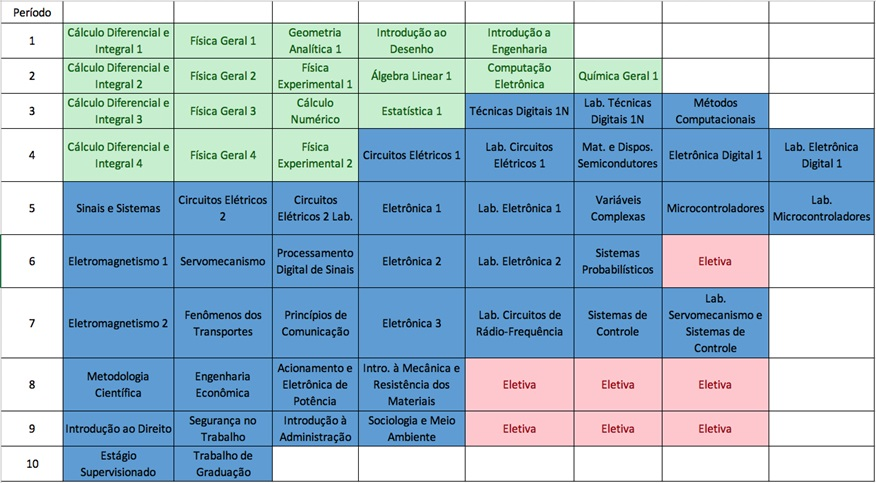
\includegraphics[width=7cm]{Ilustrações/Figura 01.jpg}\\
		{\footnotesize Fonte: Os autores.}
		\label{3.2b.eps}
	\end{center}
\end{figure}

\begin{figure}[h!]
	\caption{Disciplinas Eletivas.}
	\begin{center}
		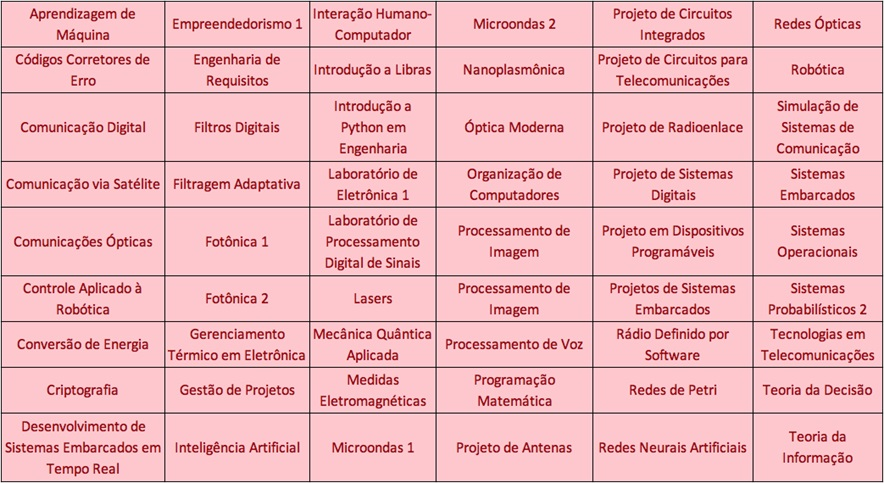
\includegraphics[width=7cm]{Ilustrações/Figura 02.jpg}\\
		{\footnotesize Fonte: Os autores.}
		\label{3.2b.eps}
	\end{center}
\end{figure}

\begin{figure}[h!]
	\caption{Organização da estrutura curricular do perfil 4507 de Engenharia Eletrônica.}
	\begin{center}
		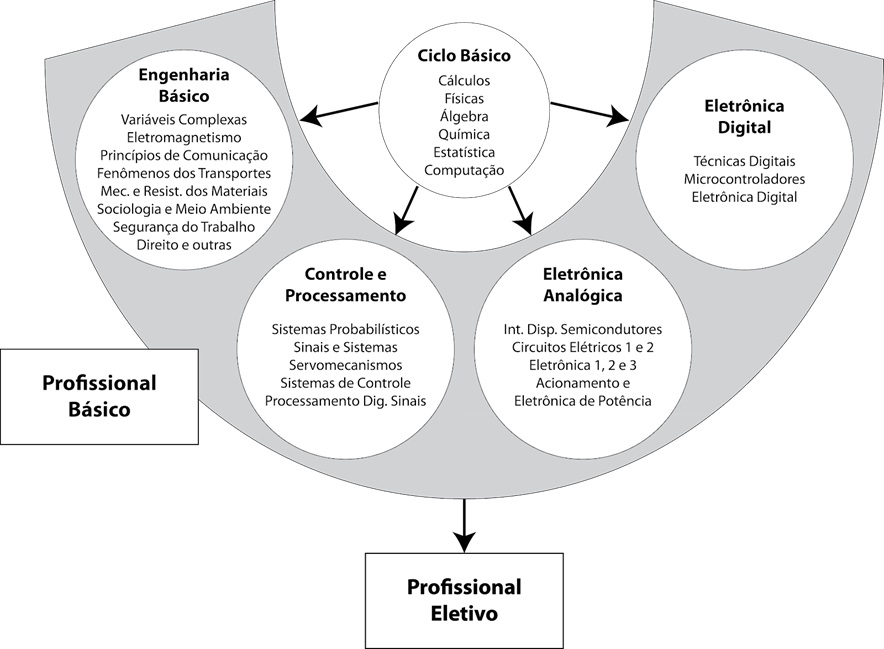
\includegraphics[width=7cm]{Ilustrações/Figura 03.jpg}\\
		{\footnotesize Fonte: Os autores.}
		\label{3.2b.eps}
	\end{center}
\end{figure}

\begin{figure}[h!]
	\caption{Disciplinas obrigatórias do ciclo profissional e suas interdependências (perfil 4507 de Engenharia Eletrônica).}
	\begin{center}
		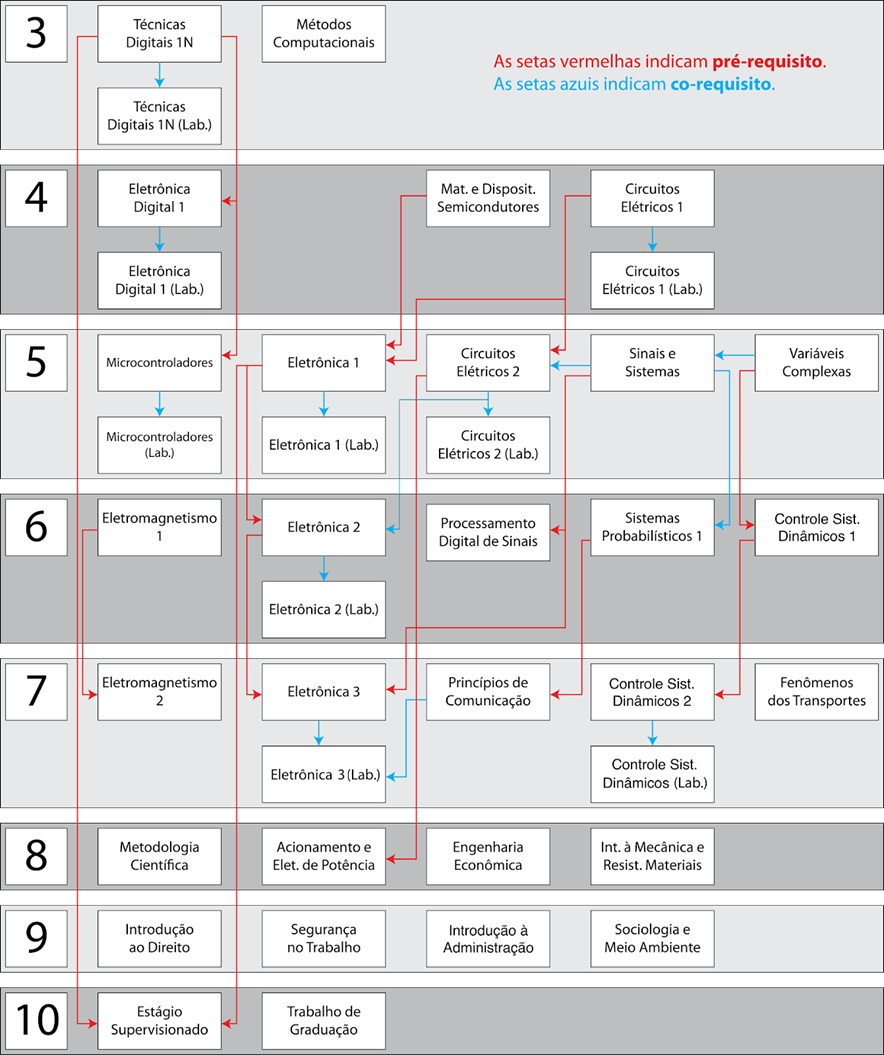
\includegraphics[width=7cm]{Ilustrações/Figura 04.jpg}\\
		{\footnotesize Fonte: Os autores.}
		\label{3.2b.eps}
	\end{center}
\end{figure} %Gerar o Capítulo 11
  \chapter{Título}
\label{cap5}
 %Gerar o Capítulo 12
  \chapter{Título}
\label{cap5}
 %Gerar o Capítulo 13
  \chapter{Título}
\label{cap5}
 %Gerar o Capítulo 14
  \chapter{Título}
\label{cap5}
 %Gerar o Capítulo 15
  \chapter{Título}
\label{cap5}
 %Gerar o Capítulo 16
  \chapter{Título}
\label{cap5}
 %Gerar o Capítulo 17
  \chapter{Título}
\label{cap5}
 %Gerar o Capítulo 18
  \backmatter
  \bibliography{Arquivos/DES}
  
  \appendix % Coloque % nesta linha caso não tenha Apêndices
  \addcontentsline{toc}{chapter}{Apêndices}%

\chapter{Título do Apêndice A}

Morbi nunc tellus, molestie et urna quis, blandit dapibus felis. Morbi semper condimentum nulla, in mattis nulla lobortis eget. Cras pretium dapibus ullamcorper. Morbi porta quis dui non volutpat. Donec feugiat sem risus. Fusce cursus neque quis molestie accumsan. Quisque lobortis purus orci, sed placerat nulla sodales vitae. Proin condimentum, nibh in aliquet mollis, eros orci dictum libero, id congue erat neque nec nulla.

Quisque sem tortor, lacinia nec tincidunt eu, efficitur vel ex. In nec leo quis justo condimentum vulputate vel ut lorem. Integer eu metus quis mi dignissim sodales. Phasellus vestibulum ex vitae nisl interdum, ut fringilla arcu dapibus. Suspendisse tristique sed nisi quis ullamcorper. Proin eu tincidunt massa.
 % Coloque % nesta linha caso não tenha o Apêndice A
  \chapter{Título do Apêndice B}

Morbi nunc tellus, molestie et urna quis, blandit dapibus felis. Morbi semper condimentum nulla, in mattis nulla lobortis eget. Cras pretium dapibus ullamcorper. Morbi porta quis dui non volutpat. Donec feugiat sem risus. Fusce cursus neque quis molestie accumsan. Quisque lobortis purus orci, sed placerat nulla sodales vitae. Proin condimentum, nibh in aliquet mollis, eros orci dictum libero, id congue erat neque nec nulla.

Quisque sem tortor, lacinia nec tincidunt eu, efficitur vel ex. In nec leo quis justo condimentum vulputate vel ut lorem. Integer eu metus quis mi dignissim sodales. Phasellus vestibulum ex vitae nisl interdum, ut fringilla arcu dapibus. Suspendisse tristique sed nisi quis ullamcorper. Proin eu tincidunt massa.
 % Coloque % nesta linha caso não tenha o Apêndice B
  %(Se precisar, crie o arquivo Arquivos/ApendiceC para o apêndice C e assim por diante e inclua uma linha para cada apêndice adicionado)
  
  \anexos  % Coloque % nesta linha caso não tenha anexos
  \addcontentsline{toc}{chapter}{Anexos}%

\chapter{Título do Anexo A}

Morbi nunc tellus, molestie et urna quis, blandit dapibus felis. Morbi semper condimentum nulla, in mattis nulla lobortis eget. Cras pretium dapibus ullamcorper. Morbi porta quis dui non volutpat. Donec feugiat sem risus. Fusce cursus neque quis molestie accumsan. Quisque lobortis purus orci, sed placerat nulla sodales vitae. Proin condimentum, nibh in aliquet mollis, eros orci dictum libero, id congue erat neque nec nulla.

Quisque sem tortor, lacinia nec tincidunt eu, efficitur vel ex. In nec leo quis justo condimentum vulputate vel ut lorem. Integer eu metus quis mi dignissim sodales. Phasellus vestibulum ex vitae nisl interdum, ut fringilla arcu dapibus. Suspendisse tristique sed nisi quis ullamcorper. Proin eu tincidunt massa.
 % Coloque % nesta linha caso não tenha o Anexo A
  \chapter{Título do Anexo B}

Morbi nunc tellus, molestie et urna quis, blandit dapibus felis. Morbi semper condimentum nulla, in mattis nulla lobortis eget. Cras pretium dapibus ullamcorper. Morbi porta quis dui non volutpat. Donec feugiat sem risus. Fusce cursus neque quis molestie accumsan. Quisque lobortis purus orci, sed placerat nulla sodales vitae. Proin condimentum, nibh in aliquet mollis, eros orci dictum libero, id congue erat neque nec nulla.

Quisque sem tortor, lacinia nec tincidunt eu, efficitur vel ex. In nec leo quis justo condimentum vulputate vel ut lorem. Integer eu metus quis mi dignissim sodales. Phasellus vestibulum ex vitae nisl interdum, ut fringilla arcu dapibus. Suspendisse tristique sed nisi quis ullamcorper. Proin eu tincidunt massa.
 % Coloque % nesta linha caso não tenha o Anexo B
  %(Se precisar, crie o arquivo Arquivos/AnexoC para o anexo C e assim por diante e inclua uma linha para cada anexo adicionado)
  
\end{document}
